As we shall see the transition into relativistic quantum mechanics is highly non-trivial; in the sense that we don't simply add a new term onto our expressions that accounts for the relativistic effects. This lecture is meant as a very brief overview/introduction to quantum field theory, and so does not claim to be self contained in any sense. The main idea we want to highlight is how the ideas change once we start accounting for relativistic effects, and what the repercussions of those changes are. 

\subsection{Heuristic Derivation of the Schr\"{o}dinger Equation}

Schr\"{o}dinger recognised that he could obtain the Schr\"{o}dinger equation from the \emph{classical} energy-momentum relation
\bse 
E = \frac{p^2}{2m} + V,
\ese 
using the substitutions 
\bse 
E \squiggle i\hbar\partial_t, \qquad \qquad P_a \squiggle -i\hbar\partial_a
\ese 
giving 
\bse 
i\hbar\partial_t\psi = -\frac{\hbar^2}{2m}\partial_a\partial^a\psi + V\psi,
\ese 
for $\psi:\R^3\to\C$. 

If we want to get the probabilistic interpretation that quantum mechanics is built on, we need to introduce an object that
\ben[label=(\roman*)]
\item Is non-negative definite, 
\item Integrates to unity,
\item This integral doesn't change in time. 
\een 
As we have been using all along the such needed object is 
\bse 
\rho := |\psi|^2.
\ese 

We might ask ourselves `How does one come up with the idea to such an object?', the answer for which comes from the following. 

Firstly its clear that $\rho\geq 0$, by definition of the inner product. We can also always arrange for the integral over all space to be unity by normalisation. Now consider the Schr\"{o}dinger equation and its complex conjugate
\bi{rCl}
i\hbar\partial_t\psi & = & -\frac{\hbar^2}{2m}\partial_a\partial^a\psi + V\psi \\
-i\hbar\partial_t\overline{\psi} & = & -\frac{\hbar^2}{2m}\partial_a\partial^a\overline{\psi} + V\overline{\psi}.
\ei 
If we multiply the former from the right by $\overline{\psi}$ and the latter from the left by $\psi$, then subtract the two results we arrive, after rearranging a bit, at 
\bi{rCl}
\big[ (\partial_t\psi)\overline{\psi} + \psi(\partial_t\overline{\psi}) \big] & = & \frac{i\hbar}{2m} \big[ \psi(\partial_a\partial^a\overline{\psi}) - (\partial_a\partial^a\psi)\overline{\psi} \big] \\
\partial_t(\psi\overline{\psi}) & = & \frac{i\hbar}{2m}\partial_a \big[ \psi(\partial^a\overline{\psi}) - (\partial^a\psi)\overline{\psi}\big].
\ei
Then defining 
\bse 
\rho := \psi\overline{\psi}, \qquad \qquad j^a := -\frac{i\hbar}{2m} \big[ \psi(\partial^a\overline{\psi}) - (\partial^a\psi)\overline{\psi}\big],
\ese 
we arrive at the continuity equation
\bse 
\partial_t\rho + \partial_aj^a = 0,
\ese 
from which it follows that 
\bi{rCl}
\partial_t \int_{\R^3}d^3x \rho(x) & = & \int_{\R^3} d^3x (\partial_t\rho)(x) \\
& = & \int_{\R^3} d^3x (\partial_aj^a)(x) \\
& = & 0,
\ei
where we have used the fact that we are integrating over all of $\R^3$ (which has no boundary/surface) with the fact that $\partial_aj^a$ is a purely surface term. 

\subsection{Heuristic Derivation of the Relativistic Schr\"{o}dinger Equation (Klein-Gordan Equation)}

A note is made on the structural difference between non-relativistic spacetime and the spacetime of general relativity. For a much deeper discussion of this the reader is directed to Dr. Schuller's International Winter School on Gravity and Light\footnote{Available via \href{https://www.youtube.com/watch?v=7G4SqIboeig&t=3811s}{YouTube}.}

Schro\"{o}dinger, quite courageously, tried to apply the method of the previous section to the relativistic energy-momentum relation ($c=1$ here),
\bse
E^2 = p^2 + m^2,
\ese 
which gives 
\bse 
-\hbar^2\partial_t^2 = -\hbar^2\partial_a\partial^a + m^2,
\ese 
which, after rearranging, gives the so-called \emph{Klein-Gordan equation}\footnote{It is named such as Oskar Klein and Walter Gordan also arrived at this result after Schro\"{o}dinger, and proceeded to try and interpret it as the description of relativistic electrons, which we shall see shortly is not the case.}
\bse 
(\Box +m^2)\phi = 0,
\ese 
where we have introduced the d'Alembert operator 
\bse 
\Box := \partial_t^2 - \partial_a\partial^a.
\ese 

The question we now have to ask is `can we still obtain some probability interpretation using $\phi$?' The answer is no, as we shall now show. 

In correlation to the non-relativistic case, in order to ensure the integral is a constant in time, we wish to find a $J^{\mu}$ such that 
\bse 
\partial_{\mu}J^{\mu} = \partial_0J^0 + \partial_aJ^a = 0.
\ese 
Again similarly to before, by considering the Klein-Gordan equation and its complex conjugate we arrive at 
\bse 
J^{\mu} := (\partial^{\mu}\phi)\overline{\psi} - \psi (\partial^{\mu}\overline{\psi}),
\ese 
and Gauss' theorem tells us that the \emph{only} candidate for the probability amplitude $\rho$ is 
\bse 
\rho := J^0 := (\partial^0\phi)\overline{\psi} - \psi (\partial^0\overline{\psi}).
\ese 
This all looks fine, in fact it looks exactly like the non-relativistic case. However there is one subtle, yet highly important, difference. In the Schr\"{o}dinger equation we had only first order time derivatives, whereas the Klein-Gordan equation is second order in time derivatives. This means that for the latter we can prescribe as initial conditions not only $\phi(t)$ but its derivative $(\partial_t\phi)(t)$ at some time. We can thus choose these initial conditions such that $\rho<0$ at some time, which violates the interpretation of $\rho$ as a probability density. This is a problem that cannot be removed at this level, the reason for which we shall soon see.

\br 
Historically, Schr\"{o}dinger actually arrived at the relativistic equation first (as he knew this was ultimately where he wanted to go), however when running into the problem highlighted above he decided instead to consider the non-relativistic case and ended up with the Schr\"{o}dinger equation.
\er 

\br 
Note some people often refer to the time and spatial derivatives being on an \emph{equal footing} in the Klein-Gordan equation. This is a highly misleading choice of words. They are not on an equal footing, as the temporal derivatives come with a positive sign, whereas the spatial ones come with a negative sign. This is not just some little difference to be brushed over. Indeed, without this minus sign stems from Maxwell's equations, and without it the Klein-Gordan equation would be physically useless; the gist being that if time and space were on an equal footing then we would not be able to predict the future, which is the main driving force of physics. What people should say is that they are on a \emph{similiar} footing. 
\er 

\subsection{Dirac Equation}

So, as we have seen, it is this second derivative that causes us the problems, so the natural question is `How do we avoid it?' The immediate answer is to try considering 
\bse 
E = \sqrt{p^2+m^2},
\ese 
and then using the substitutions as above. However this is no better as now the RHS is the square root of a differential operator, and so in the expansion about $m^2$ we will end up with a theory with infinite spatial derivative order. Not good at all! 

Dirac then asked the question `What if I use a different substitution prescription such that the whole of the RHS becomes a single order derivative?' Following this thought, after several calculations, he arrives at the so-called \emph{Dirac equation} 
\bse 
(i\gamma^\mu\partial_\mu - m\b1_4)\Psi = 0,
\ese 
where the $\gamma^{\mu}$ are $4\times4$ matrices satisfying the anticommutation relation
\bse 
\{\gamma^{\mu},\gamma^{\nu}\} := \gamma^{\mu}\gamma^{\nu} + \gamma^{\mu}\gamma^{\nu} = 2\eta^{\mu\nu},
\ese 
known as the \emph{Dirac algebra}, where $\eta^{\mu\nu}$ is the Minkowski metric given by\footnote{Using the (-,+,+,+) signature.} 
\bse 
\eta^{\mu\nu} = \text{diag}(-1,1,1,1).
\ese 
The vector $\Psi$ here is a 4 component object known as a spinor, where (after some work) we can think of two of the components being a particle and the other two being the associated antiparticle. 

So the Dirac equation introduces antimatter into the mix, however it turns out that it still doesn't fix the probability problem addressed by the Klein-Gordan equation!

\subsection{The Deep Route of the Problem}

It turns out the problem stems from perhaps the most well-known equation in the world... $E=mc^2$, which tells us that we need not conserve particle number. For example the interaction between two particles could result in any number of resulting particles (provided the energy is in sufficiently large) 

\begin{center}
\begin{tikzpicture}
\draw[thick, ->] (1,0) -- (2,0);
\draw[thick, ->] (3,-2) -- (3,-1);
\draw[thick, ->] (3,0) -- (4.5,2.5);
\draw[thick, ->] (3,0) -- (5,1.5);
\draw[thick, ->] (3,0) -- (4.5,-1);
\draw[thick, ->] (3,0) -- (5,0);
\draw[fill=white] (3,0) circle [radius=1];
\draw[pattern=north west lines, pattern color=blue] (3,0) circle [radius=1];
\end{tikzpicture}
\end{center}

If this information is contained within $E=mc^2$, it is also contained in the relativistic energy-momentum equation $E^2= p^2 +m^2c^4$, and so we were unjustified to look for an equation in the relativistic context that describes \emph{one} (or any fixed number) of particles. In other words, our theory needs to account for this non-conservation of particle number, including have no particles (i.e. the vacuum). Mathematically the idea is to construct a direct sum of Hilbert spaces, each of which describes a different number of particles. This is known as the \emph{Fock space}, 
\bse 
\cF := \C \oplus \cH \oplus (\cH\otimes\cH) \oplus (\cH\otimes\cH\otimes\cH) \oplus ...
\ese 

We can then construct the inner product on $\cF$ from the inner products on the Hilbert spaces, all of which are obtained from the inner product on $\cH$. That is if $\psi,\varphi\in\cF$ given by 
\bi{rCl}
\psi & = & a_0 \oplus a_1 \psi_1 \oplus \sum_{ij} a_2^{ij} (\psi_{2i}\otimes\psi_{2j}) \oplus  ... \\
\varphi & = & b_0 \oplus b_1 \varphi_1 \oplus \sum_{ij} b_2^{ij} (\varphi_{2i} \otimes\varphi_{2j}) \oplus ...,
\ei
then the inner product is given by 
\bse 
\braket{\psi}{\varphi} = \overline{a_0}b_0 + \overline{a_1}b_1\braket{\psi_1}{\varphi_1}_{\cH} + \sum_{ijk\ell} \overline{a^{ij}_2}b^{k\ell}_2 \braket{\psi_{2i}\otimes\psi_{2j}}{\varphi_{2k}\otimes\varphi_{2\ell}}_{\cH\otimes\cH} + ...
\ese 

\br 
For the Klein-Gordan equation it is actually the \emph{symmetrised} tensor products we need, giving this symmetric Fock space
\bse 
\odot \cF := \C \oplus (\cH\odot\cH) \oplus (\cH\odot\cH\odot\cH) \oplus ...,
\ese 
and it describes \emph{bosonic} systems. 

Similarly for the Dirac equation we require the \emph{anti-symmetrised} tensor product, giving 
\bse 
\wedge \cF := \C \oplus (\cH\wedge\cH) \oplus (\cH\wedge\cH\wedge\cH) \oplus ...,
\ese 
which describes \emph{fermionic} systems.
\er 

We claim that once you lift the Klein-Gordan and Dirac equations onto their respective Fock spaces, that the problem of negative probability density vanishes. 

\subsection{Feynman Diagrams}

Richard Feynman developed a pictorial representation of the highly complicated interaction of particles. The basic idea is to take a perturbation expansion of the interaction and represent each order by a set of diagrams. The order of the diagram is associated with the number of so-called \emph{vertices} present. 

For example the first few terms for the process of electron-electron scattering would be drawn as:

% I had trouble with the Tikz-Feyman package in this file, so I drew this elsewhere and imported it as a picture.
\begin{center}
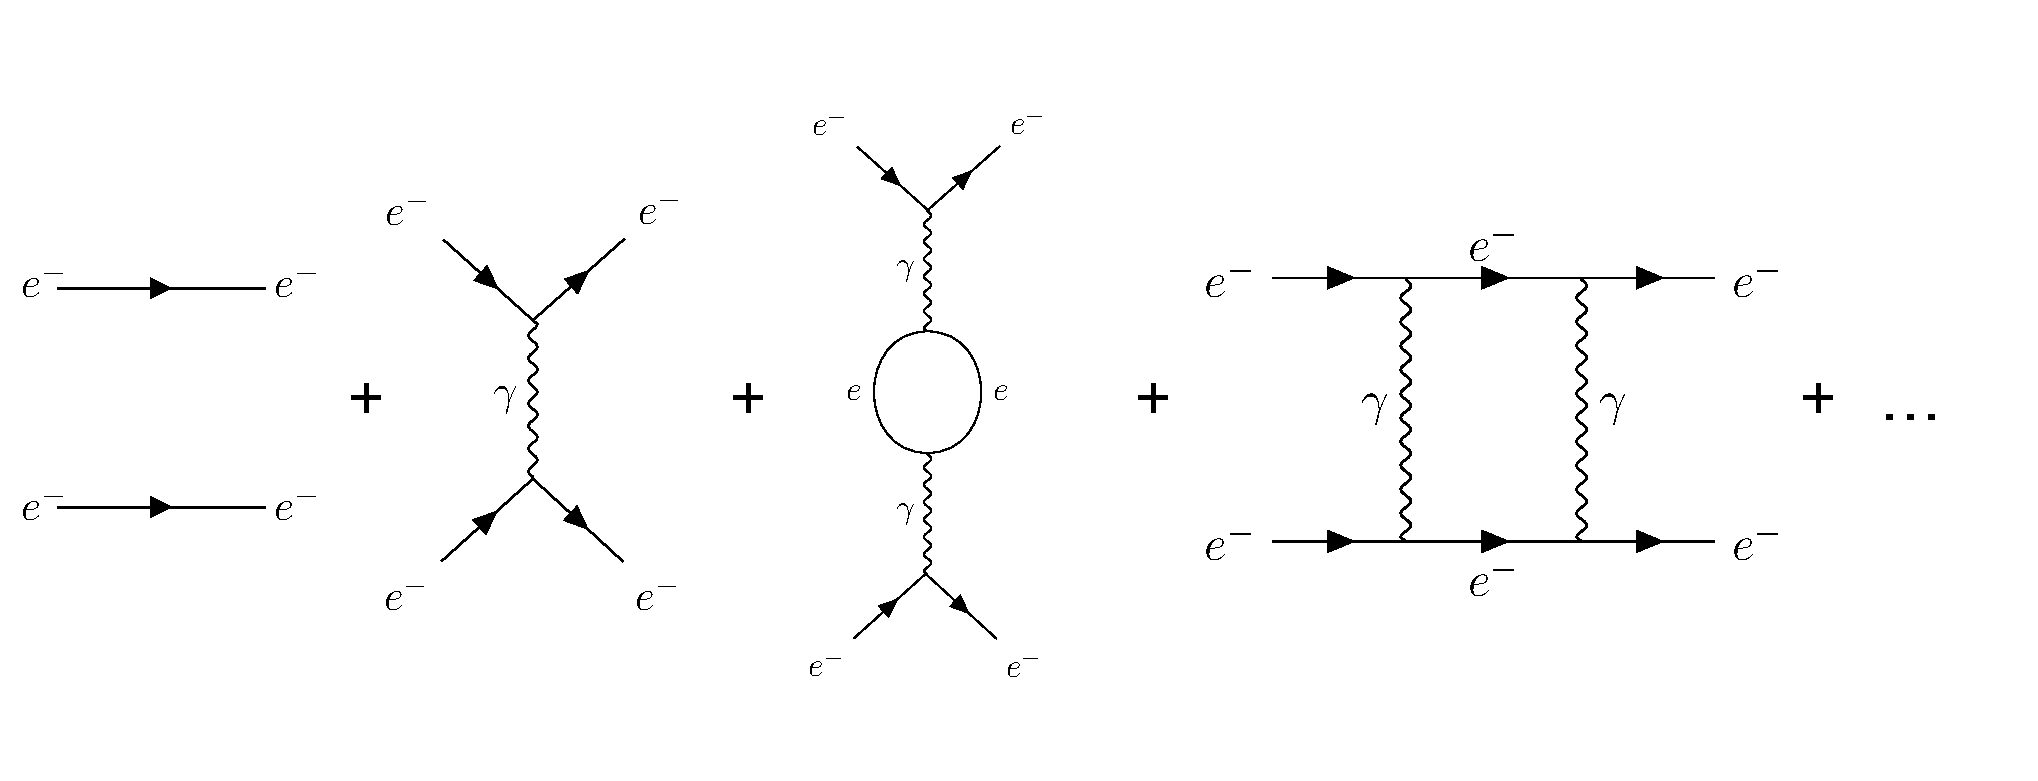
\includegraphics[scale=0.45, origin=c]{graphics/Feynman.pdf}
\end{center}

The first diagram (which has no vertices) is the zeroth order diagram, the second one (with two vertices) is the second order diagram and the last two (which both have 4 vertices) are the fourth order diagrams. The furthest most left and right arrows (i.e. the ones that have a non-vertexed end) are known as \emph{external lines}, and the other ones are known as \emph{internal lines}. Particles represented by internal lines are often referred to \emph{virtual} particles. 

\br 
One should be careful when it comes to drawing the arrows on the internal lines, however, as (unless the rest of the diagram indicates otherwise) we could have a particle or an antiparticle (whose arrow points the opposite way). It is for this reason that the so-called \emph{loop} in the third diagram does not have arrows. On the final diagram we do draw the arrows, as conservation of electric charge forces us to ensure our virtual particles are electrons (not positrons, the anti-electron). 

Note also on loop internal lines we have simply written $e$ and not $e^-$ or $e^+$ (the positron), this further indicates that we do not know which is which, only that one must be an electron and the other a positron. 
\er 

Mathematically Feynman diagrams correspond to integral equations, and there is a set of rules (cleverly named \emph{Feyman Rules}) which tell you how to convert the diagrams into these integrals. They are a indispensable tool when it comes to studying relativistic particle physics, as not only are they quicker to draw then writing out integrals, they have some incredibly elegant properties (such as so-called \emph{crossing symmetry}) which make the calculations significantly easier. However, we shall not go into any more detail here; the unfamiliar reader is directed to the massive resource of information in textbooks/on the internet. 